\section{Introducción}
\begin{frame}{¿Qué esperar del taller?}
\begin{columns}
\column[t]{0.5\textwidth}
    \begin{itemize}
         \item Aprender el paradigma de \href{https://iquilezles.org/articles/nvscene2008/rwwtt.pdf}{Rendering Worlds With Two Triangles}.
         \item Parte del \href{https://www.smu.edu/meadows/newsandevents/news/2023/what-is-creative-coding}{creative codding}: intersección entre el arte y la ciencia.
         \item Un poco de \href{https://www.khronos.org/opengl/wiki/OpenGL_Shading_Language}{GLSL}, y las matemáticas básicas para hacer un \href{https://www.khronos.org/opengl/wiki/Portal:OpenGL_Shading_Language/Fragment_Shader}{fragment shader} en el paradigma.
     \end{itemize}
\column[t]{0.5\textwidth}
\begin{figure}[htp]
 \centering
 \begin{subfigure}[b]{0.42\textwidth}
   
\includegraphics[width=\textwidth]{img/Demo/SwirlyWhirly}
   \caption{\href{https://www.shadertoy.com/view/X3dBRr}{Swirly Whirly}}
 \end{subfigure}
~
 \begin{subfigure}[b]{0.42\textwidth}
   \includegraphics[width=\textwidth]{img/Demo/SelfieGirl}
   \caption{\href{https://www.shadertoy.com/view/WsSBzh}{Selfie Girl}}
 \end{subfigure}
\\
 \begin{subfigure}[b]{0.42\textwidth}
   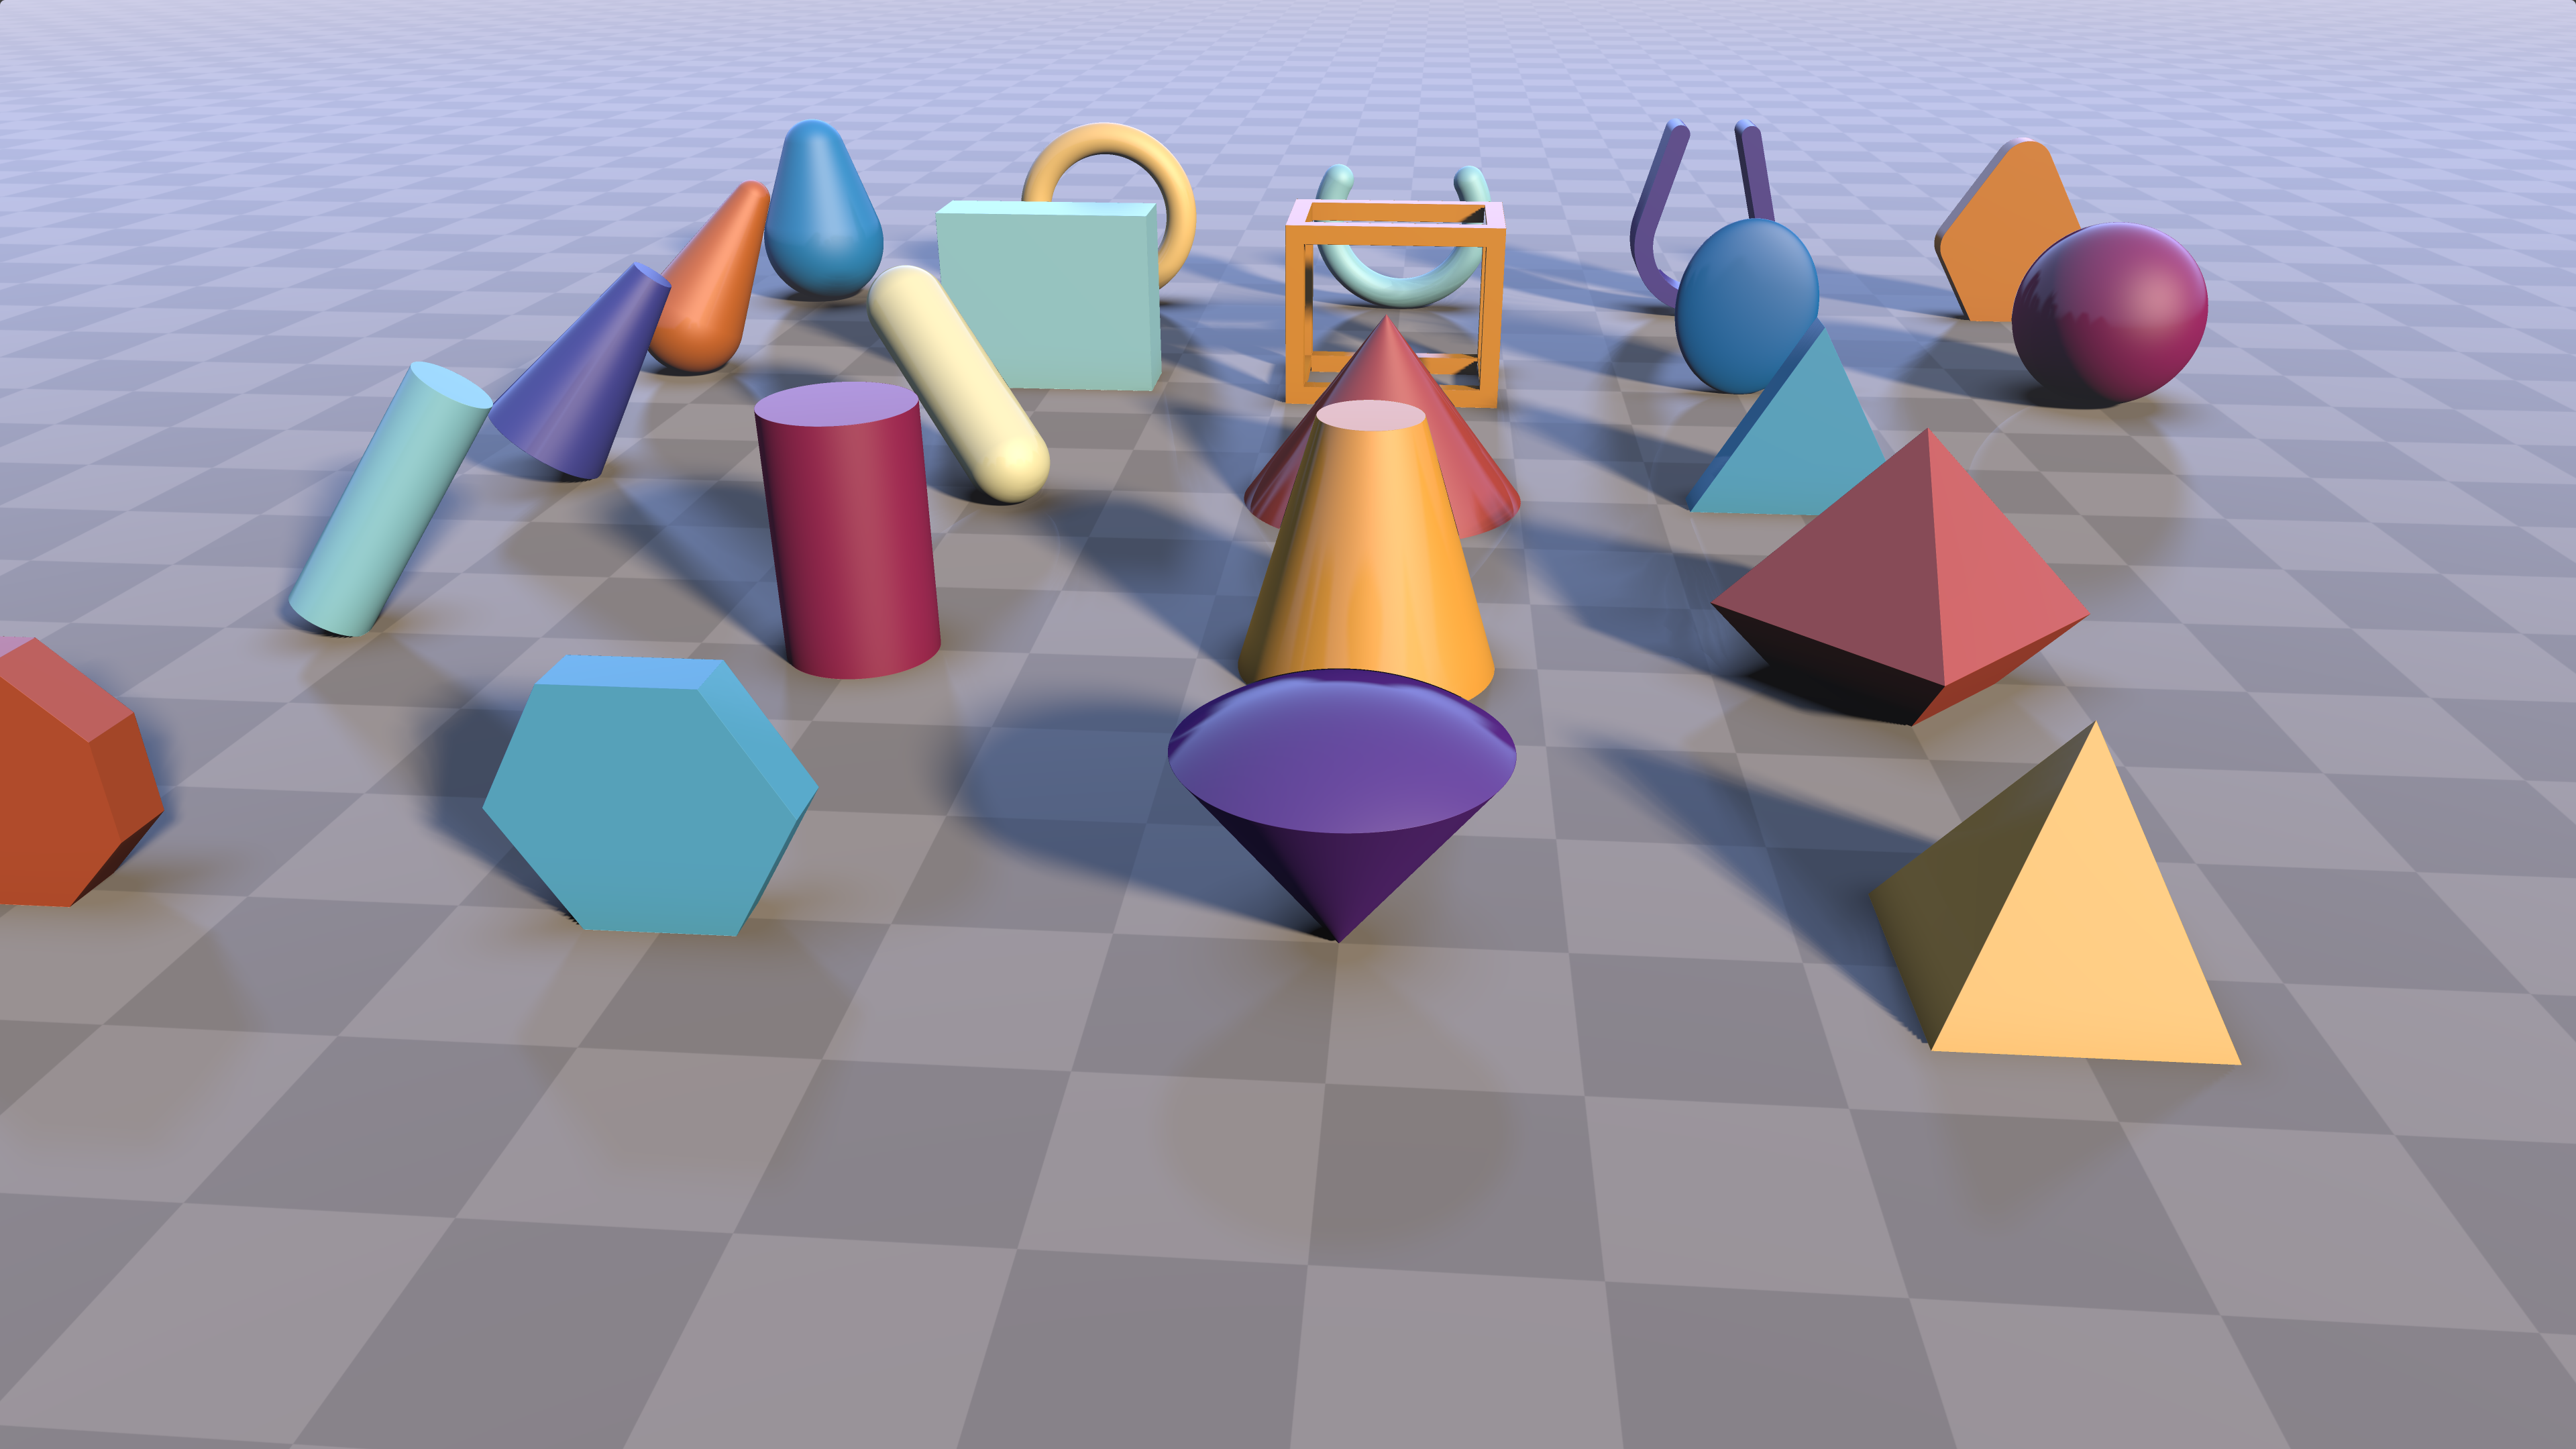
\includegraphics[width=\textwidth]{img/Demo/Raymarching-Primitives}
   \caption{\href{https://www.shadertoy.com/view/Xds3zN}{Raymarch Primitives}}
 \end{subfigure}
~
 \begin{subfigure}[b]{0.42\textwidth}
   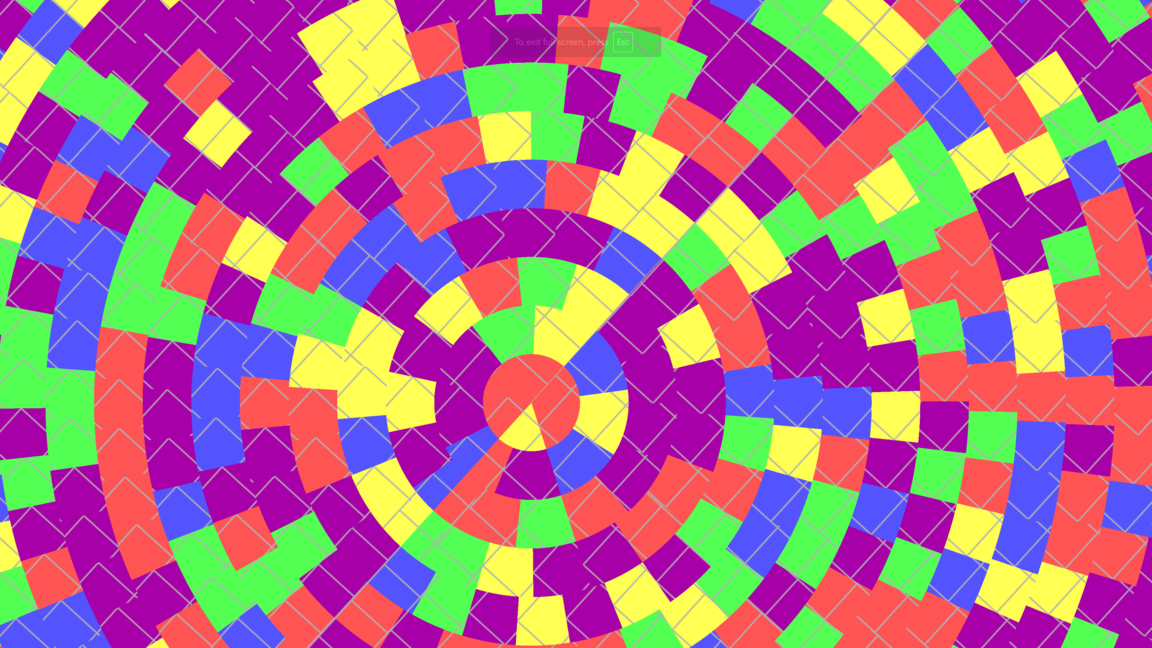
\includegraphics[width=\textwidth]{img/Demo/AnimatedCentricMosaicTiles}
   \caption{\href{https://www.shadertoy.com/view/43tfRr}{Centric Mosaic Tiles}}
 \end{subfigure}
 \caption{Propiedad de los respectivos autores.}
\end{figure}
\end{columns}
\end{frame}

\begin{frame}{¿Qué \emph{no es} éste taller?}
    No es un curso \emph{completo} de \say{Graficación por Computadora}.
    Mas aun, no vamos a enseñar a hacer gráficas por computadora de manera correcta.
    \begin{itemize}
         \item Usar este paradigma \alert{es un juego}. No se usa en producción.
         \item Los shaders que vamos a escribir son ineficientes.
         \item El código puede ser ofuscado.
     \end{itemize}
     Por razones de tiempo, tampoco enseñaremos todo lo que hay en el truco.
     \begin{itemize}
        \item Este es un taller \alert{básico} de shaders de juguete (Shadertoy).
        \item Revisaremos un conjunto de técnicas simples.
        \item Recuerda: hacer shaders complejos, requiere de experiencia, creatividad y tiempo.
    \end{itemize}
    \begin{block}{Inteligencia Artificial (IA)}
    	Aunque es posible usar IA para escribir shaders, en este taller no la usaremos, ni promoveremos su uso.
    \end{block}
\end{frame}

\begin{frame}{¿Qué puedo aprovechar de éste taller?}
    \begin{itemize}
         \item Aprender una manera de expresión artística usando programación.
         \item Un excelente ejercicio para fomentar la creatividad.
         \item Una forma de practicar, aplicar y mejorar tus conocimientos de matemáticas y de computación.
         \item Un medio de compartir con una comunidad (Shadertoy tiene elementos de red social).
         \item Se convierte en un hobby productivo.
     \end{itemize}
     
     \begin{block}{Graficación por Computadora}
         \begin{itemize}
            \item Una probadita para saber si estas interesado en tomar un curso formal después.
            \item Si ya tomaste el curso, es un \emph{hack} muy elegante que seguramente no se te había ocurrido.
            \item Muchos profesionales del área lo practican como hobby.
        \end{itemize}  
    \end{block}
\end{frame}

\begin{frame}{Acerca de mí}
    \begin{columns}
\column[t]{0.5\textwidth}
        \begin{figure}[htb]
            \centering
            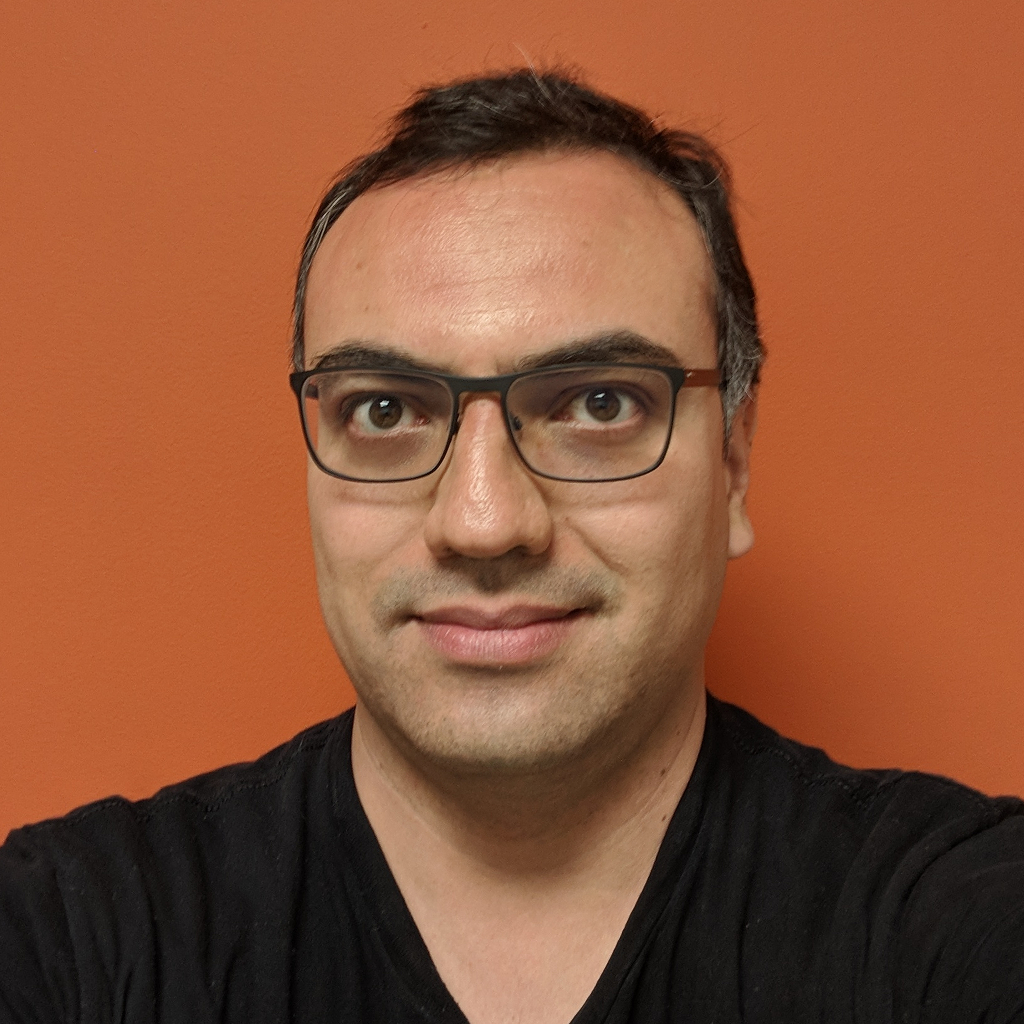
\includegraphics[width=0.6\textwidth]{img/Avatar12}
            \caption{Dr. Jorge Antonio García Galicia.}
        \end{figure}
\column[t]{0.5\textwidth}
     \begin{itemize}
         \item \href{https://mac.acatlan.unam.mx/}{Licenciatura} y \href{https://www.pcic.unam.mx/}{maestría} en la \href{https://www.unam.mx/}{UNAM}.
         \item \href{https://polytechnic.purdue.edu/degrees/phd-technology}{Doctorado} en \href{https://www.purdue.edu/}{Purdue University}.
         \item Hice una pasantía en \href{https://research.adobe.com/}{Adobe} y trabajé en \href{https://www.nvidia.com/}{Nvidia}.
         \item He dado clases en \href{https://www.acatlan.unam.mx/}{Acatlán} y fui ayudante en \href{https://www.fciencias.unam.mx/directorio/63922}{Ciencias} y en \href{https://polytechnic.purdue.edu/}{Purdue}.
         \item Actualmente soy SWE en \href{https://about.google/}{Google}.
         \item Tengo mas de 15 años de experiencia en Tecnología.
     \end{itemize}
\end{columns}
\end{frame}

\begin{frame}{Mi experiencia con gráficos}
\begin{columns}
\column[t]{0.5\textwidth}
    \begin{itemize}
         \item Tres tesis que tienen que ver con \href{https://en.wikipedia.org/wiki/Computer_graphics}{Graficación por Computadora}.
         \item Publicado en \href{https://direct.mit.edu/leon}{Leonardo}, \href{https://www.siggraph.org/}{SIGGRAPH} y en \href{https://www.eg.org/wp/eurographics-publications/}{Eurographics}.
         \item Trabajé en el driver de \href{https://www.opengl.org/}{OpenGL} y en \href{https://stadia.google.com/gg/}{Stadia}.
         \item Actualmente trabajo en \href{https://www.android.com/xr/}{AndroidXR}.
         \item Provengo de una familia de artistas.
     \end{itemize}
\column[t]{0.5\textwidth}
\begin{figure}[htp]
 \centering
 \begin{subfigure}[b]{0.4\textwidth}
   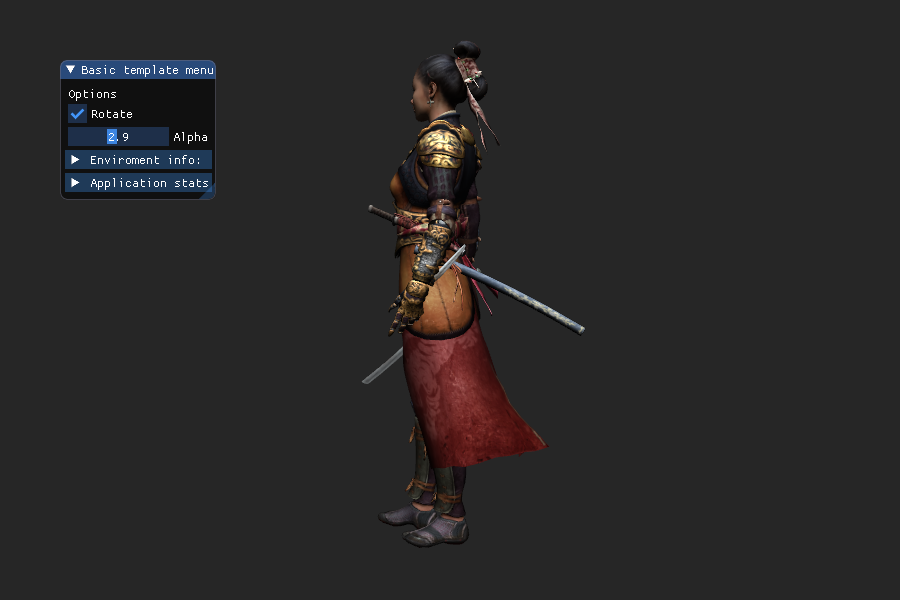
\includegraphics[width=\textwidth]{img/menuTemplate}
 \end{subfigure}
~
 \begin{subfigure}[b]{0.4\textwidth}
   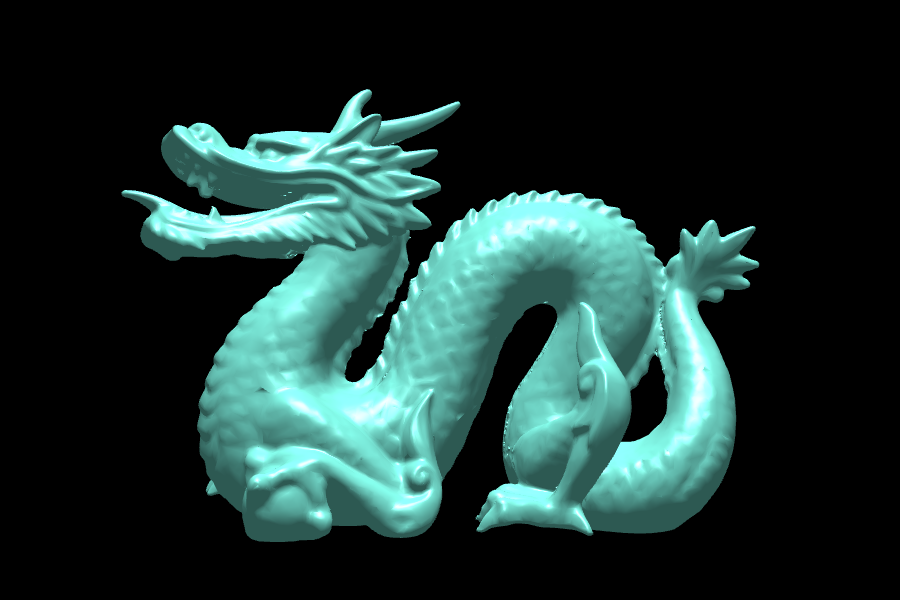
\includegraphics[width=\textwidth]{img/completo}
 \end{subfigure}
\\
 \begin{subfigure}[b]{0.4\textwidth}
   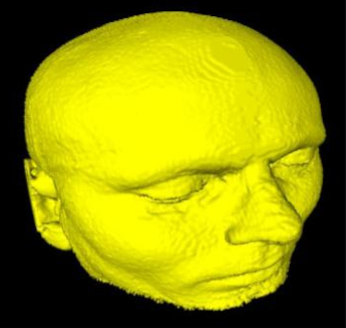
\includegraphics[width=\textwidth]{img/master}
 \end{subfigure}
~
\begin{subfigure}[b]{0.4\textwidth}
   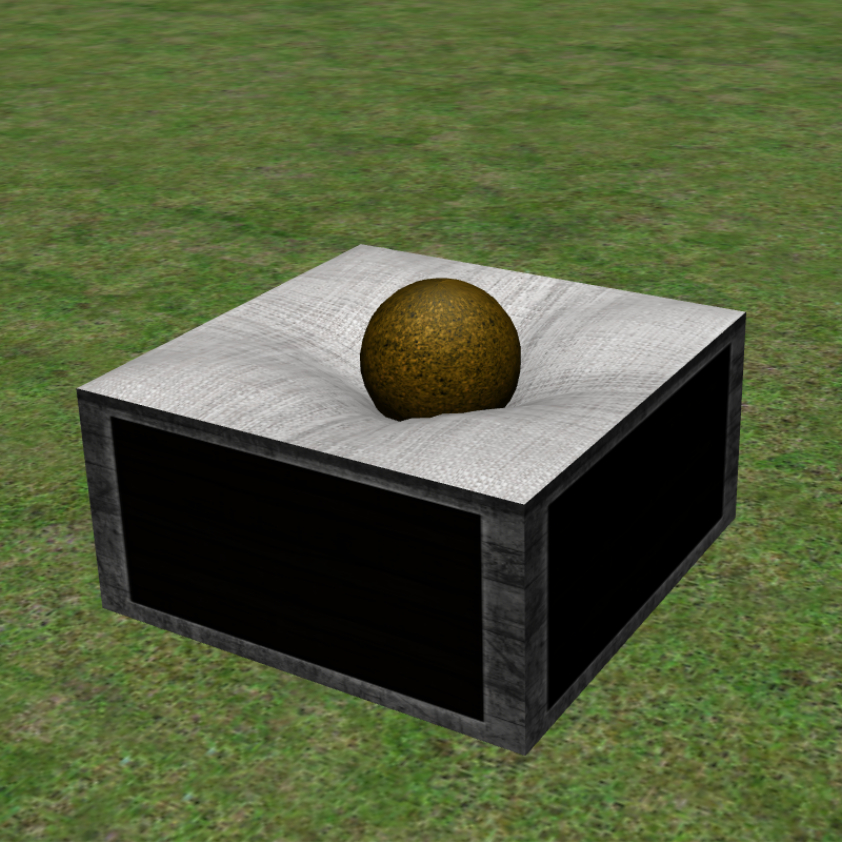
\includegraphics[width=\textwidth]{img/bachelor_thesis}
 \end{subfigure}
 
\end{figure}
\end{columns}
\end{frame}
